\documentclass[10pt,a4paper]{amsart}
\usepackage[margin=19mm]{geometry}
\usepackage{amsmath,amssymb,mathtools}
\usepackage[scr=rsfs,cal=euler]{mathalfa}
\usepackage{xfrac}
\usepackage[unicode,hidelinks,bookmarks=false]{hyperref}
\newcommand{\ie}{i.e.\ }
\newcommand{\cf}{cf.\ }
\newcommand{\resp}{respectively\ }
\newcommand{\Subsection}{\subsection}
\providecommand{\nobreakdash}{\nobreak\hbox{-}}
\setlength{\emergencystretch}{2em}
\multlinegap0pt
\usepackage{tikz}
\usepackage{float}
\usepackage{amssymb}
\usepackage[shortlabels]{enumitem}
\newtheorem{lemma}{Lemma}
\newtheorem{claim}{Claim}
\newtheorem{subproof}{Subproof}
\title{Erd\H{o}s-Hajnal conjecture beyond five-vertex graphs}
\author{Shenwei Huang, Yiao Ju, Yidong Zhou}
\date{Source: arXiv:2606.06258v3 (CC BY 4.0)}
\begin{document}
\maketitle

\noindent\emph{Source and licence.} Erd\H{o}s-Hajnal conjecture beyond five-vertex graphs. Version arXiv:2606.06258v3 (CC BY 4.0), distributed by arXiv under the Creative Commons Attribution 4.0 International licence, http://creativecommons.org/licenses/by/4.0/, as recorded in the arXiv licence metadata for this exact version and shown on the abstract page https://arxiv.org/abs/2606.06258v3. Full licence notice: \texttt{licenses/arxiv-2606.06258-CC-BY-4.0.txt}.\par\smallskip

\noindent\textit{Editorial scope.} Counted unit: the article's lemma lem:coro-lem (source0.tex lines 1789--1801). The article's complete original proof of it is delivered with it (source0.tex lines 1802--1968, one \texttt{proof} environment of 167 lines). No mathematics is written, repaired or re-derived: the statement and the proof are the article's own lines, in the article's own notation, and no retained line is substituted or re-flowed.  Retained uncounted as the source-local context the proof needs: lines 1451--1462; lines 1472--1485.  Nothing was omitted from any retained span, so the package carries no omission record.  No retained line contains a citation, so the wrapper carries no bibliography and no bibliography entry.  The retained lines contain the article's own diagram code, which the wrapper typesets with the standard tikz packages; no image file is delivered and the package declares no asset dependency.  Editorial formatting only, in addition: an AMS \texttt{amsart} preamble that restates the article's own declarations and macros used by the retained lines, namely the environments \texttt{lemma}, \texttt{claim}, \texttt{subproof} on separate counters, together with the standard packages those lines need.  The retained environments print in this document as Lemma 1, Claim 1, Subproof 1 in order of appearance, whereas the article prints the same items with the numbering of its own full document.  The complete native source of the article as distributed in the arXiv e-print for this exact version is bundled unchanged as \texttt{sources/202171/source0.tex}.
        \begin{lemma}\label{clm:property of levels}
            Suppose that $\mathcal{L}$ is a blockade such that each block of $\mathcal{L}$ is connected (anti-connected). 
            Then  
            \begin{itemize}
                \item[$(1)$] Each block of $\mathcal{L}/\mathcal{M}$ is also connected (resp. anti-connected).
                
                \item[$(2)$] Each two blocks of $\mathcal{L}$ that are contained in different blocks of $\mathcal{L}/\mathcal{M}$ are pure to each other.
                
                \item[$(3)$] If there are a block $D$ of $\mathcal{L}/\mathcal{M}$ and a vertex $u\notin D$ that is mixed on $D$ but is pure to each block of $\mathcal{L}$ contained in $D$, then there are two mixed blocks of $\mathcal{L}$ contained in $D$ such that $u$ is complete to one of the blocks and anti-complete to the other.
    
            \end{itemize}
        \end{lemma}

        \begin{lemma}\label{clm:inductive}
            Suppose that $\mathcal{L}$ is a blockade in $G$ such that each block of $\mathcal{L}$ is connected (anti-connected). 
            If there are two mixed blocks $D_1,D_2$ of $\mathcal{L}/\mathcal{M}$ and three vertices $x,y,u\notin D_1\cup D_2$ such that 
            \begin{itemize}
                \item $x,y$ are two non-adjacent vertices that are complete to $D_1\cup D_2$,
                \item $u\in N(x)\setminus N(y)$ is complete to $D_1$ but is anti-complete to $D_2$, and
                \item no vertex in $D_1$ can mix on $D_2$,
            \end{itemize}
            then there are two mixed blocks $A_1,A_2$ of $\mathcal{L}$ that contained in $D_1$ and three vertices $x',y',u'\notin A_1\cup A_2$ such that 
            \begin{itemize}
                \item[$(1)$] $x',y'$ are two non-adjacent vertices that are complete to $A_1\cup A_2$ and
                \item[$(2)$] $u'\in N(x')\setminus N(y')$ is complete to $A_1$ but is anti-complete to $A_2$.  
            \end{itemize}
        \end{lemma}

    \begin{lemma}\label{lem:coro-lem}
        Let $G$ be a co-Bird-free graph with a $(\ell,w)$-comb $((a_i,B_i),i\in[\ell])$ in $G$ and a vertex $v\in V(G)\setminus(\{a_i:i\in[\ell]\}\cup\bigcup_{i\in[\ell]}B_i)$ such that $v$ is complete to $\bigcup_{i\in[\ell]}B_i$ and anti-complete to $\{a_i:i\in[\ell]\}$. 
        For each $i\in[\ell]$, $B_i$ can be partitioned into $X_i,Y_i$ such that 
        \begin{itemize}
            \item[$(1)$] $Y_i$ is $E$-graph-free;  
            \item[$(2)$] $X_i$ can be partitioned into $(A^i_1,\ldots, A^i_{t_i})$ such that 
            \begin{itemize}
                \item[$(2.1)$] $(A^i_1,\ldots, A^i_{t_i})$ is a pure blockade; 
                \item[$(2.2)$] the pattern of $(A^i_1,\ldots, A^i_{t_i})$, whose vertex set consists of all blocks of $(A^i_1,\ldots, A^i_{t_i})$ and two vertices are adjacent if and only if their corresponding blocks are complete to each other, is $E$-graph-free; 
                \item[$(2.3)$] for each $j\in [t_i]$ and every vertex $u\in \bigcup_{k\in [\ell]\setminus \{i\}} B_k$, $u$ is pure to $A^i_j$.
            \end{itemize}
        \end{itemize} 
    \end{lemma}

    \begin{proof}
        We begin with a useful claim. 
        \begin{claim}\label{clm:a vertex mixed on a path via bird}
            Let $S$ be an induced subgraph of $G$ and $x,y\in V(G)\setminus V(S)$ be two non-adjacent vertices complete to $S$. 
            For every induced subgraph $H$ of $S$, there is no $u\in N(x)\setminus N(y)$ for which either of the following holds. 
            \begin{itemize}
                \item[$(1)$] $H$ is $P_2+P_1$ and $u$ is mixed on the $P_2$ but is anti-complete to the $P_1$.  
                \item[$(2)$] $H$ is $P_3+P_1$ and $u$ is adjacent to the $P_1$ and two consecutive vertices of the $P_3$ but is anti-complete to the remaining vertex of the $P_3$.  
            \end{itemize} 
        \end{claim}
        
        \begin{subproof}[Proof of Claim \ref{clm:a vertex mixed on a path via bird}]
            Let $u\in N(x)\setminus N(y)$ be a vertex. 
            Suppose first that $H$ is $P_2+P_1$ with edge $ab$ and the isolated vertex $c$. 
            If $u$ is adjacent to $a$ but is non-adjacent to $b$ and $c$, then $\{x,y,u,a,b,c\}$ induces a co-Bird (see Figure \ref{fig:co-Bird in claim 5.2.1}), a contradiction. 
            This proves Claim \ref{clm:a vertex mixed on a path via bird} (1). 

            Now we suppose that $H$ is $P_3+P_1$ with induced path $a-b-c$ and the isolated vertex $d$. 
            If $u$ is adjacent to $b,c,d$ but is non-adjacent to $a$, then $\{y,u,a,b,c,d\}$ induces a co-Bird (see Figure \ref{fig:co-Bird in claim 5.2.1}), a contradiction. 
            This proves Claim \ref{clm:a vertex mixed on a path via bird} (2). 
        \end{subproof}
        
        \begin{figure}[h!]
        \centering
        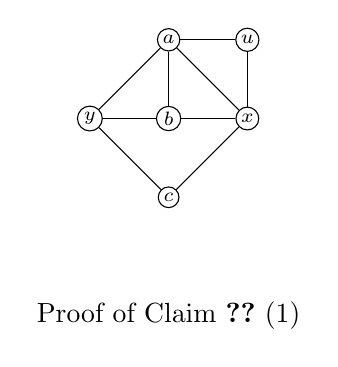
\begin{tikzpicture}[scale=1]
        \tikzstyle{vertex}=[circle, draw, fill=white, inner sep=1pt, minimum size=5pt]
        
            \node[vertex](1) at (0,1){\scriptsize $a$};
            \node[vertex](2) at (0,0){\scriptsize $b$};
            \node[vertex](3) at (0,-1){\scriptsize $c$};
            
            \node[vertex](4) at (1,0){\scriptsize $x$};
            \node[vertex](5) at (-1,0){\scriptsize $y$};
            \node[vertex](6) at (1,1){\scriptsize $u$};

            
            \node at (0,-2.5) {Proof of Claim \ref{clm:a vertex mixed on a path via bird} (1)};
            
            \foreach \from/\to in {1/2}
            \draw (\from) -- (\to);

            \foreach \from/\to in {4/1,4/2,4/3}
            \draw (\from) -- (\to);

            \foreach \from/\to in {5/1,5/2,5/3}
            \draw (\from) -- (\to);

            \foreach \from/\to in {6/1,6/4}
            \draw (\from) -- (\to);

        \end{tikzpicture}
        \hspace{10mm}
        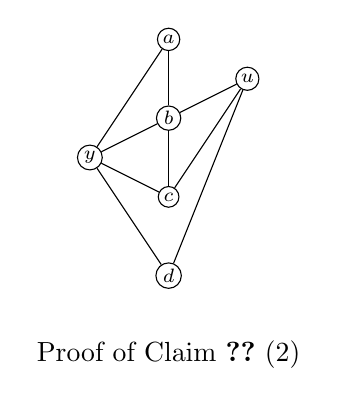
\begin{tikzpicture}[scale=1]
        \tikzstyle{vertex}=[circle, draw, fill=white, inner sep=1pt, minimum size=5pt]
        
            \node[vertex](1) at (0,1.5){\scriptsize $a$};
            \node[vertex](2) at (0,0.5){\scriptsize $b$};
            \node[vertex](3) at (0,-0.5){\scriptsize $c$};
            \node[vertex](4) at (0,-1.5){\scriptsize $d$};
            
            \node[vertex](5) at (-1,0){\scriptsize $y$};
            \node[vertex](6) at (1,1){\scriptsize $u$};

            
            \node at (0,-2.5) {Proof of Claim \ref{clm:a vertex mixed on a path via bird} (2)};
            
            \foreach \from/\to in {1/2,2/3}
            \draw (\from) -- (\to);

            \foreach \from/\to in {5/1,5/2,5/3,5/4}
            \draw (\from) -- (\to);

            \foreach \from/\to in {6/3,6/2,6/4}
            \draw (\from) -- (\to);

        \end{tikzpicture}
        \caption{Induced co-Birds in the proof of Claim \ref{clm:a vertex mixed on a path via bird}.}
        \label{fig:co-Bird in claim 5.2.1}
    \end{figure}
        
        \begin{claim}\label{clm:homo structure}
            If $x,y$ are two non-adjacent vertices complete to an induced $E$-graph,
            then every vertex $u\in N(x)\setminus N(y)$ is pure to this $E$-graph. 
            In particular, for every vertex $u\in \bigcup_{k\in [\ell]\setminus \{i\}} B_k$, $u$ is pure to every induced $E$-graph in $B_i$. 
        \end{claim}
        \begin{subproof}[Proof of Claim \ref{clm:homo structure}]
            Suppose to the contrary that there is a vertex $u\in N(x)\setminus N(y)$ that is mixed on an induced $E$-graph. 
            Let $P=v_1-v_2-v_3-v_4-v_5$ be the induced $P_5$ contained in this $E$-graph and $v_3'$ be the vertex adjacent to $v_3$. 
            
            Suppose first that $u$ is complete to $P$.  
            By Claim \ref{clm:a vertex mixed on a path via bird} (2) with $H$ induced by $\{v_3',v_3,v_4,v_1\}$, we have $u$ is adjacent to $v_3'$.   
            Then $u$ is complete to this $E$-graph, a contradiction. 
            So $u$ is not complete to $P$. 
            Now we suppose that $u$ is anti-complete to $P$. 
            By Claim \ref{clm:a vertex mixed on a path via bird} (1) with $H$ induced by $\{v_1,v_3,v_3'\}$, we have $u$ is not adjacent to $v_3'$. 
            It follows that $u$ is anti-complete to this $E$-graph, a contradiction. 
            So $u$ is not anti-complete to $P$. 

            Therefore, we may assume $u$ is mixed on $P$.
            Suppose first that $u$ is mixed on $v_1v_2$. 
            By Claim \ref{clm:a vertex mixed on a path via bird} (1), $u$ is adjacent to each of $v_3',v_4,v_5$.
            If $u$ is adjacent to $v_1$ but is not adjacent to $v_2$, then $u$ is adjacent to $v_3$
            by Claim \ref{clm:a vertex mixed on a path via bird} (2) with $H$ induced by $\{v_1,v_3,v_4,v_5\}$.
            Then the $\{v_2,v_3,v'_3,v_5\}$ contradicts 
            Claim \ref{clm:a vertex mixed on a path via bird} (2).
            So we may assume that $u$ is adjacent to $v_2$ but is not adjacent to $v_1$. 
            By Claim \ref{clm:a vertex mixed on a path via bird} (1) with $H$ induced by $\{v_1,v_3,v_3'\}$, $u$ is adjacent to $v_3$. Then $\{v_1,v_2,v_3,v_5\}$ contradicts Claim \ref{clm:a vertex mixed on a path via bird} (2).
            This proves that $u$ is pure to $v_1v_2$.
            By symmetry, $u$ is pure to $v_4v_5$. 

            If $u$ is adjacent to $v_1,v_2,v_4,v_5$, then $u$ is non-adjacent to $v_3$ and then $\{v_1,v_2,v_3,v_5\}$ contradicts Claim \ref{clm:a vertex mixed on a path via bird} (2).
            If $u$ is non-adjacent to $v_1,v_2,v_4,v_5$, then $u$ is adjacent to $v_3$ and so $\{v_2,v_3,v_5\}$ contradicts Claim \ref{clm:a vertex mixed on a path via bird} (1).
            So we may assume that $u$ is adjacent to $v_1,v_2$ but is non-adjacent to $v_4,v_5$. 
            By Claim \ref{clm:a vertex mixed on a path via bird} (1) with $H$ induced by $\{v_2,v_3,v_5\}$, $u$ is adjacent to $v_3$. 
            By Claim \ref{clm:a vertex mixed on a path via bird} (2) with $H$ induced by $\{v_1,v_3',v_3,v_4\}$, $u$ is not adjacent to $v_3'$, which gives a contradiction by Claim \ref{clm:a vertex mixed on a path via bird} (1) with $H$ induced by $\{v_3,v_3',v_5\}$. 
            This proves the first statement of the claim.
            
            The second statement of Claim \ref{clm:homo structure} follows immediately with $(x,y)$ replaced by $(v,a_i)$. 
            This completes the proof of Claim \ref{clm:homo structure}. 
        \end{subproof}
        
        Now we are ready to define $X_i,Y_i$ and $(A^i_1,\ldots, A^i_{t_i})$. 
        Let $X_i\subseteq B_i$ be the set of all vertices contained in some induced $E$-graph in $B_i$ and $Y_i=B_i\setminus X_i$. So $Y_i$ is $E$-graph-free.   
        This proves Lemma \ref{lem:coro-lem} (1). 
        For any two vertices $d,d'\in X_i$, we say $d,d'$ have {\em relation $\mathcal{R}$} if and only if there is a vertex sequence $d=d_1,d_2,\ldots,d_n=d'$ such that for each $k\in [n-1]$, $d_k$ and $d_{k+1}$ are contained in the same induced $E$-graph in $B_i$. 
        It is easy to check that $\mathcal{R}$ is an equivalence relation on $X_i$. 
        Let $\mathcal{L}^1$ be the blockade whose blocks are equivalence classes of $\mathcal{R}$. 
        Since $E$-graph is anti-connected, each block of $\mathcal{L}^1$ is anti-connected. 
        For each $s\geq 2$, let $\mathcal{L}^{s}=\mathcal{L}^{s-1}/\mathcal{M}$. 
        Note that $\mathcal{L}^{s}$ is different from $\mathcal{L}^{s-1}$ if and only if there are two mixed blocks in $\mathcal{L}^{s-1}$.
        Since $X_i$ is finite, there is an integer $q$ such that $\mathcal{L}^{q}$ is a pure blockade. 
        Set $(A^i_1,\ldots, A^i_{t_i}):=\mathcal{L}^{q}$ and  
        this proves Lemma \ref{lem:coro-lem} (2.1). 
        If there is an induced $E$-graph such that each vertex of this $E$-graph is contained in a different block of $(A^i_1,\ldots,A^i_{t_i})$, then these vertices should have been in the same block of $\mathcal{L}^1$, a contradiction. 
        This proves Lemma \ref{lem:coro-lem} (2.2).
        It remains to prove Lemma \ref{lem:coro-lem} (2.3).
      
        \begin{claim}\label{clm:homo blocks}
            For every $s\in[q]$, every block $L$ of $\mathcal{L}^s$ and every vertex $u\in \bigcup_{k\in [\ell]\setminus \{i\}} B_k$, $u$ is pure to $L$.
        \end{claim}
        \begin{subproof}[Proof of Claim \ref{clm:homo blocks}]
            We prove this claim by induction on $s$. 
            If $s=1$, then this claim follows immediately from Claim \ref{clm:homo structure} with $(x,y,u)=(v,a_i,u)$. 
            So we may assume that $s\ge 2$ and this claim holds for $s-1$.

            Suppose to the contrary that there is a vertex $u\in \bigcup_{k\in [\ell]\setminus \{i\}} B_k$ that is mixed on $L$.  
            By the inductive hypothesis, $u$ is pure to each block of $\mathcal{L}^{s-1}$. 
            By Lemma \ref{clm:property of levels} (3), there are two mixed blocks of $\mathcal{L}^{s-1}$ contained in $L$ such that $u$ is complete to one of these two blocks but is anti-complete to the other one. 
            Suppose that for each fixed $i\in [s]$, there are two mixed blocks $D_1,D_2$ of $\mathcal{L}^i$ and three vertices $x,y,z$ with $z\in N(x)\setminus N(y)$ such that $x,y$ are complete to $D_1\cup D_2$ and $z$ is complete to $D_1$ and anti-complete to $D_2$. If $b_1\in D_1$ mixes on $D_2$, then $b_1$ mixed on a non-edge $b_2b'_2\in D_2$ by anti-connectivity. 
            By Claim \ref{clm:a vertex mixed on a path via bird} (1) with $(H,x,y,z)=(\{b_1b_2\}+b_2',x,y,z)$, we obtain a contradiction.

            By applying Lemma \ref{clm:inductive} repeatedly, beginning with $(x,y,u)=(v,a_i,u)$, where each application of Lemma \ref{clm:inductive} preserves the same hypotheses until reaching $\mathcal{L}^1$, there are two mixed blocks $A_1,A_2$ of $\mathcal{L}^1$ and three vertices $x',y',u'\notin A_1\cup A_2$ such that 
            \begin{itemize}
                \item $x',y'$ are two non-adjacent vertices that are complete to $A_1\cup A_2$, and
                \item $u'\in N(x')\setminus N(y')$ is complete to $A_1$ but is anti-complete to $A_2$.  
            \end{itemize}
            
            So we may assume that there is a vertex $u_2\in A_2$ mixed on $A_1$. 
            By Claim \ref{clm:homo structure} with $(x,y,u)=(y',u',u_2)$, $u_2$ is pure to every induced $E$-graph of $A_1$. 
            Since $A_1$ is an equivalence class of $\mathcal{R}$, $u_2$ is pure to $A_1$, a contradiction.  
            
            This complete the proof of Claim \ref{clm:homo blocks}. 
        \end{subproof} 

        By Claim \ref{clm:homo blocks} with $s=q$, Lemma \ref{lem:coro-lem} (2.3) holds.
        This completes the proof of Lemma \ref{lem:coro-lem}. 
    \end{proof}

\end{document}
